\documentclass{article}
\pagenumbering{arabic}

\usepackage{url}
\usepackage{color}
\usepackage{verbatim}
\usepackage{tikz}
\usepackage{gnuplot-lua-tikz}

\usepackage{xspace}

%\usepackage[utf8]{inputenc}
%\usepackage{fontspec}
\usepackage{pgfplots}

\usepackage[procnames]{listings}
\lstset{ %
  backgroundcolor=\color{gray98},    % choose the background color; you must add \usepackage{color} or \usepackage{xcolor}
  basicstyle=\tt\small, % \prettysmall      % the size of the fonts that are used for the code
  breakatwhitespace=false,          % sets if automatic breaks should only happen at whitespace
  breaklines=true,                  % sets automatic line breaking
  showlines=true,                  % sets automatic line breaking
  captionpos=b,                     % sets the caption-position to bottom
  commentstyle=\color{gray30},      % comment style
  extendedchars=true,               % lets you use non-ASCII characters; for 8-bits encodings only, does not work with UTF-8
  frame=single,                     % adds a frame around the code
  keepspaces=true,                  % keeps spaces in text, useful for keeping indentation of code (possibly needs columns=flexible)
  keywordstyle=\color{amblu},       % keyword style
  procnamestyle=\color{amred},       % procedures style
  language=[95]fortran,             % the language of the code
  numbers=left,                     % where to put the line-numbers; possible values are (none, left, right)
  numbersep=5pt,                    % how far the line-numbers are from the code
  numberstyle=\tiny\color{gray20}, % the style that is used for the line-numbers
  rulecolor=\color{gray20},          % if not set, the frame-color may be changed on line-breaks within not-black text (e.g. comments (green here))
  showspaces=false,                 % show spaces everywhere adding particular underscores; it overrides 'showstringspaces'
  showstringspaces=false,           % underline spaces within strings only
  showtabs=false,                   % show tabs within strings adding particular underscores
  stepnumber=2,                     % the step between two line-numbers. If it's 1, each line will be numbered
  stringstyle=\color{amblu},       % string literal style
  tabsize=2,                        % sets default tabsize to 2 spaces
  % title=\lstname,                    % show the filename of files included with \lstinputlisting; also try caption instead of title
  procnamekeys={call}
}

\usepackage{color}
\definecolor{gray98}{rgb}{0.98,0.98,0.98}
\definecolor{gray20}{rgb}{0.20,0.20,0.20}
\definecolor{gray25}{rgb}{0.25,0.25,0.25}
\definecolor{gray16}{rgb}{0.161,0.161,0.161}
\definecolor{gray60}{rgb}{0.6,0.6,0.6}
\definecolor{gray30}{rgb}{0.3,0.3,0.3}
\definecolor{bgray}{RGB}{248, 248, 248}
\definecolor{amgreen}{RGB}{77, 175, 74}
% \definecolor{amblu}{RGB}{72, 88, 102}
\definecolor{amblu}{RGB}{55, 126, 184}
\definecolor{amred}{RGB}{228,26,28}
\definecolor{amyellow}{RGB}{237,177,32}
\definecolor{ampurple}{RGB}{126,47,142}
\newcommand{\mye}[1]{\textcolor{amyellow}{#1}\xspace}
\newcommand{\mgr}[1]{\textcolor{amgreen}{#1}\xspace}
\newcommand{\mbl}[1]{\textcolor{amblu}{#1}\xspace}
\newcommand{\mre}[1]{\textcolor{amred}{#1}\xspace}
\newcommand{\mbk}[1]{\textcolor{black}{#1}\xspace}
\newcommand{\mbp}[1]{\textcolor{ampurple}{#1}\xspace}

% This version: August 21st, 2008

%%%%%%%%%%%%%%%%%%%%%%%%%%%%% packages %%%%%%%%%%%%%%%%%%%%%%%%%%%%%%

\usepackage{savesym}
%\usepackage{repdefs,latexsym,longtable,cite}
\usepackage{latexsym,longtable,cite}
\usepackage{accents}
\usepackage{varioref}
\savesymbol{dddot}
\savesymbol{ddddot}
\usepackage{amsmath}
\restoresymbol{TXF}{dddot}
\restoresymbol{TXF}{ddddot}
\usepackage{stfctitlepage}
\usepackage{amssymb}
\usepackage{subfigure}
\usepackage{algorithmic}
\usepackage{algorithm}
\usepackage[usenames,dvipsnames]{pstricks}
\usepackage{epsfig}
\usepackage{pst-grad} % For gradients
\usepackage{pst-plot} % For axes
\usepackage[section]{placeins}
\usepackage{lscape}

%%%%%%%%%%%%%%%%%%%%%%% definitions from repdefs %%%%%%%%%%%%%%%%%%%%%

% formatting

\textwidth  16.17cm 
\textheight 23.4cm
\oddsidemargin -0.2mm 
\evensidemargin -0.2mm
\def\baselinestretch{1.1} 
\topmargin -8.4mm 
\renewcommand{\textfraction}{0.05}
\setlength{\unitlength}{1mm}

% sections

\newcommand{\resetcounters}{\setcounter{equation}{0} \setcounter{figure}{0} 
 \setcounter{table}{0}}
\newcommand{\numsection}[1]{\section{#1}\resetcounters}

% Equations, tables and figures numbered by chapter and section

\renewcommand{\theequation}{\arabic{section}.\arabic{equation}}
\renewcommand{\thetable}{\arabic{section}.\arabic{table}}
\renewcommand{\thefigure}{\arabic{section}.\arabic{figure}}

% displayed equations

\newcommand{\eqn}[2]{\begin{equation}\label{#1}{#2}\end{equation}}
\newcommand{\disp}[1]{\[{#1}\]}
\newcommand{\tim}[1]{\;\; \mbox{#1} \;\;}
\newcommand{\rim}[1]{\;\;\; \mbox{#1} \;\;\;}

% arrays etc

\newcommand{\vect}[1]{\left(\begin{array}{c}#1\end{array}\right)}
\newcommand{\mat}[2]{\left(\begin{array}{#1}#2\end{array}\right)}
\newcommand{\matinv}[2]{\left(\begin{array}{#1}#2\end{array}\right)^{-1}}
\newcommand{\arr}[2]{\begin{array}{#1}#2\end{array}}

% shorthand for itemize, etc

\newcommand{\ite}[1]{\begin{itemize}{#1}\end{itemize}}
\newcommand{\enu}[1]{\begin{enumerate}{#1}\end{enumerate}}
\newcommand{\des}[1]{\begin{description}{#1}\end{description}}

% mathematics

\renewcommand{\Re}{\hbox{I\hskip -1.5pt R}}
\newcommand{\smallRe}
     {\mbox{\raisebox{-0.8pt}{\footnotesize I\hskip -1.5pt R\hskip -0.5pt}}}
\newcommand{\mininx}[1]{ {\renewcommand{\arraystretch}{0.8} 
                     \begin{array}[t]{c} 
                     \mbox{minimize} \vspace*{-1mm} \\ 
                     \mbox{ $\scriptstyle x \in \smallRe^n #1 $ } 
                     \end{array} \;} }
\newcommand{\minin}[1]{ {\renewcommand{\arraystretch}{0.8} 
                     \begin{array}[t]{c} 
                     \mbox{minimize} \vspace*{-1mm} \\ 
                     \mbox{ $\scriptstyle #1 $ } 
                     \end{array} \;} }
\newcommand{\eqdef}{\stackrel{\rm def}{=}}
\newcommand{\bigsum}{\displaystyle \sum}
\newcommand{\bigfrac}[2]{\displaystyle\frac{#1}{#2}}
\newcommand{\s}[1]{^{\mbox{\protect\tiny #1}}}
\newcommand{\sub}[1]{_{\mbox{\protect\tiny #1}}}
\newcommand{\st}{\,\mid\,}
\newcommand{\diag}{\mbox{diag}}

%  fractions

\newcommand{\sfrac}[2]{{\scriptstyle \frac{#1}{#2}}}
\newcommand{\half}{\sfrac{1}{2}}
\newcommand{\quarter}{\sfrac{1}{4}}
\newcommand{\eighth}{\sfrac{1}{8}}

% theorems etc

\newtheorem{theorem}{Theorem}[section]
\newtheorem{lemma}[theorem]{Lemma}
\newtheorem{corollary}[theorem]{Corollary}
\newtheorem{example}{Example}[section]
\newtheorem{defn}{Definition}[section]
\newtheorem{remark}{Remark}[section]
\newtheorem{assumption}{Assumption}[section]
\newcommand{\llem}[2]{\vspace{\baselineskip} 
 \noindent\framebox[\textwidth]{\parbox{0.95\textwidth}{
 \begin{lemma} \label{#1} \rm #2 \end{lemma} } } \vspace{\baselineskip} }
\newcommand{\lthm}[2]{\vspace{\baselineskip} 
 \noindent\framebox[\textwidth]{\parbox{0.95\textwidth}{
 \begin{theorem} \label{#1} \rm #2 \end{theorem} } } \vspace{\baselineskip} }
\newcommand{\lcor}[2]{\vspace{\baselineskip}
 \noindent\framebox[\textwidth]{\parbox{0.95\textwidth}{
 \begin{corollary} \label{#1} \rm #2 \end{corollary} } } \vspace{\baselineskip} }
\newcommand{\lassump}[2]{\vspace{\baselineskip}
 \noindent\framebox[\textwidth]{\parbox{0.95\textwidth}{
 \begin{assumption} \label{#1} \rm #2 \end{assumption} } } \vspace{\baselineskip} }
\newcommand{\ldefn}[2]{\vspace{\baselineskip}
 \noindent\framebox[\textwidth]{\parbox{0.95\textwidth}{
 \begin{defn} \label{#1} \rm #2 \end{defn} } } \vspace{\baselineskip} }

% proofs

\newcommand{\bpr}{{\bf Proof.} \hspace{1.5mm}}
\newcommand{\epr}{\hfill $\Box$ \vspace*{1em}}
\newcommand{\proof}[1]{
\begin{list}{}{
\setlength{\topsep}{0.0pt}
\setlength{\partopsep}{0.0pt}
\setlength{\leftmargin}{0.025\textwidth}
\setlength{\rightmargin}{0.5\leftmargin}
\setlength{\labelwidth}{0.5\leftmargin}
\setlength{\labelsep}{0.25\leftmargin}}
\item \bpr #1 \epr \noindent
\end{list}}

% appendix

\newcommand{\newappendixname}{A}
\newcommand{\newappendix}[1]{\renewcommand{\newappendixname}{{#1}}
 \section*{Appendix \newappendixname} 
 \resetcounters
 \renewcommand{\theequation}{\newappendixname.\arabic{equation}}
 }

% calligraphic letters

\newcommand{\calA}{{\cal A}} \newcommand{\calB}{{\cal B}}
\newcommand{\calC}{{\cal C}} \newcommand{\calD}{{\cal D}}
\newcommand{\calE}{{\cal E}} \newcommand{\calF}{{\cal F}}
\newcommand{\calG}{{\cal G}} \newcommand{\calH}{{\cal H}}
\newcommand{\calI}{{\cal I}} \newcommand{\calJ}{{\cal J}}
\newcommand{\calK}{{\cal K}} \newcommand{\calL}{{\cal L}}
\newcommand{\calM}{{\cal M}} \newcommand{\calN}{{\cal N}}
\newcommand{\calO}{{\cal O}} \newcommand{\calP}{{\cal P}}
\newcommand{\calQ}{{\cal Q}} \newcommand{\calR}{{\cal R}}
\newcommand{\calS}{{\cal S}} \newcommand{\calT}{{\cal T}}
\newcommand{\calU}{{\cal U}} \newcommand{\calV}{{\cal V}}
\newcommand{\calW}{{\cal W}} \newcommand{\calX}{{\cal X}}
\newcommand{\calY}{{\cal Y}} \newcommand{\calZ}{{\cal Z}}

% figures

\newcommand{\fig}[2]{\begin{figure}[htbp]
\begin{center} {#1} \caption{#2} \end{center} \end{figure}}
\newcommand{\figt}[2]{\begin{figure}[t]
\begin{center} {#1} \caption{#2} \end{center} \end{figure}}


%%%%%%%%%%%%%%%%%%%%%%% additional definitions %%%%%%%%%%%%%%%%%%%%%%%

\newcommand{\mycitetwo}[4]{[\citenum{#1}: #2, \citenum{#3}: #4]}
\newcommand{\mycitethree}[3]{[\citenum{#1}: #2, \citenum{#3}]}

\newcommand{\lk}{\lambda_k}
\newcommand{\lkp}{\lambda_{k+1}}
\newcommand{\dk}{\delta_k}

\newcommand{\lambdac}{\lambda\sub{C}}
\newcommand{\lambdae}{\lambda\sub{E}}
\newcommand{\lambdas}{\lambda\sub{S}}
\newcommand{\lambdal}{\lambda\sub{L}}
\newcommand{\lambdat}{\lambda\sub{T}}
\newcommand{\lambdau}{\lambda\sub{U}}
\newcommand{\xs}{x\sub{S}}
\newcommand{\alphas}{\alpha\sub{S}}
\newcommand{\thetal}{\theta\sub{L}}
\newcommand{\thetau}{\theta\sub{U}}

\newcommand{\xl}{x(\lambda)}
\newcommand{\xlt}{x^T(\lambda)}
\newcommand{\xlp}{\dot{x}(\lambda)}
\newcommand{\xlpt}{\dot{x}^T(\lambda)}
\newcommand{\xlpp}{\ddot{x}(\lambda)}
\newcommand{\xlppt}{\ddot{x}^T(\lambda)}

\newcommand{\xlz}{x^{(0)}(\lambda)}
\newcommand{\xlo}{x^{(1)}(\lambda)}
\newcommand{\xlk}{x^{(k)}(\lambda)}
\newcommand{\xlkt}{x^{(k)T}(\lambda)}
\newcommand{\xlkm}{x^{(k-1)}(\lambda)}
\newcommand{\xlkp}{x^{(k+1)}(\lambda)}
\newcommand{\xlkpt}{x^{(k+1)T}(\lambda)}
\newcommand{\xlkpp}{x^{(k+2)}(\lambda)}

\newcommand{\ylz}{y^{(0)}(\lambda)}
\newcommand{\ylk}{y^{(k)}(\lambda)}
\newcommand{\ylkt}{y^{(k)T}(\lambda)}
\newcommand{\ylkp}{y^{(k+1)}(\lambda)}
\newcommand{\ylkpt}{y^{(k+1)T}(\lambda)}
\newcommand{\ylkm}{y^{(k-1)}(\lambda)}

\newcommand{\zlz}{z^{(0)}(\lambda)}
\newcommand{\zlk}{z^{(k)}(\lambda)}
\newcommand{\zlkp}{z^{(k+1)}(\lambda)}
\newcommand{\zlkm}{z^{(k-1)}(\lambda)}

\newcommand{\Hlm}{H + \lambda M}
\newcommand{\Hlmc}{H + \lambdac M}

\newcommand{\pil}{\pi(\lambda)}
\newcommand{\pilp}{\pi^{(1)}(\lambda)}
\newcommand{\pilpp}{\pi^{(2)}(\lambda)}
\newcommand{\pilppp}{\pi^{(3)}(\lambda)}
\newcommand{\pilpppp}{\pi^{(4)}(\lambda)}

%\newcommand{\pilp}{\dot{\pi}(\lambda)}
%\newcommand{\pilpp}{\ddot{\pi}(\lambda)}
%\newcommand{\pilppp}{\dddot{\pi}(\lambda)}
%\newcommand{\pilpppp}{\ddddot{\pi}(\lambda)}

\newcommand{\pitkp}{\pi^{(2k+1)}(\lambda)}
\newcommand{\pitkpt}{\pi^{(2k+2)}(\lambda)}

\newcommand{\yl}{y(\lambda)}
\newcommand{\ylp}{\dot{y}(\lambda)}
\newcommand{\ylpt}{\dot{y}^T(\lambda)}
\newcommand{\ylpp}{\ddot{y}(\lambda)}
\newcommand{\ylppt}{\ddot{y}^T(\lambda)}

\newcommand{\zl}{z(\lambda)}
\newcommand{\zlp}{\dot{z}(\lambda)}
\newcommand{\zlpt}{\dot{z}^T(\lambda)}
\newcommand{\zlpp}{\ddot{z}(\lambda)}
\newcommand{\zlppt}{\ddot{z}^T(\lambda)}

%\newcommand{\baru}{\bar{u}}
%\newcommand{\barx}{\bar{x}}
%\newcommand{\barz}{\bar{z}}
%\newcommand{\barc}{\bar{c}}
%\newcommand{\barH}{\bar{H}}
\newcommand{\barc}{\skew4\overline c}
\newcommand{\barr}{\skew1\overline r}
\newcommand{\baru}{\skew0\overline u}
\newcommand{\barw}{\skew0\overline w}
\newcommand{\barx}{\skew1\overline x}
\newcommand{\bary}{\skew1\overline y}
\newcommand{\barz}{\skew2\overline z}
\newcommand{\barH}{\skew4\overline H}
\newcommand{\barU}{\skew1\overline U}
\newcommand{\hatH}{H\sub{S}}
\newcommand{\hatM}{M\sub{S}}
\newcommand{\hatu}{u\sub{S}}
\newcommand{\hatlambdal}{\lambda\sub{SL}}
%\newcommand{\Dlambda}{\Delta \lambda}
\newcommand{\Dlambda}{\delta}
\newcommand{\Dlambdac}{\delta\sub{C}}

 \newcommand{\mnorm}[1]{\|#1\|_M}

\newcommand{\bovt}{\sfrac{\beta}{2}}

% replace the next two by the best lower bounds for quadratic and cubic approx

\newcommand{\bestq}{-\sfrac{2}{3}}
\newcommand{\bestc}{-\sfrac{2}{5}}
\newcommand{\Real}{\mathbb{R}}

\newcommand{\ud}{\mathrm{d}}
\newcommand{\uu}{\mathbf{u}}
\newcommand{\ff}{\mathbf{f}}
\newcommand{\bb}{\mathbf{b}}
\newcommand{\dd}{\mathbf{d}}

%%%%%%%%%%%%%%%%%%%%%%%% Added by Sue %%%%%%%%%%%%%%%%%%%%%%%%%%%%%%%

\newcommand{\etl}{\eta(\lambda;\beta)}
\newcommand{\etlp}{\eta^{(1)}(\lambda;\beta)}
\newcommand{\etlpp}{\eta^{(2)}(\lambda;\beta)}
\newcommand{\etlppp}{\eta^{(3)}(\lambda;\beta)}
\newcommand{\etlpppp}{\eta^{(4)}(\lambda;\beta)}


\newcommand{\zetl}{\zeta(\lambda;\beta)}
\newcommand{\zetlp}{\zeta^{(1)}(\lambda)}
\newcommand{\zetlpp}{\zeta^{(2)}(\lambda)}
\newcommand{\zetlppp}{\zeta^{(3)}(\lambda)}
\newcommand{\zetlpppp}{\zeta^{(4)}(\lambda)}

%\newcommand{\etlp}{\dot{\eta}(\lambda)}
%\newcommand{\etlpp}{\ddot{\eta}(\lambda)}
%\newcommand{\etlppp}{\dddot{\eta}(\lambda)}
%\newcommand{\etlpppp}{\ddddot{\eta}(\lambda)}

\newcommand{\rhl}{\rho(\lambda)}
\newcommand{\rhlp}{\rho^{(1)}(\lambda)}
\newcommand{\rhlpp}{\rho^{(2)}(\lambda)}
\newcommand{\rhlppp}{\rho^{(3)}(\lambda)}
\newcommand{\rhlpppp}{\rho^{(4)}(\lambda)}

%\newcommand{\rhlp}{\dot{\rho}(\lambda)}
%\newcommand{\rhlpp}{\ddot{\rho}(\lambda)}
%\newcommand{\rhlppp}{\dddot{\rho}(\lambda)}
%\newcommand{\rhlpppp}{\ddddot{\rho}(\lambda)}

\newcommand{\pilb}{\pi(\lambda; \beta)}
\newcommand{\pilbp}{\pi^{(1)}(\lambda; \beta)}
\newcommand{\pilbpp}{\pi^{(2)}(\lambda; \beta)}
\newcommand{\pilbppp}{\pi^{(3)}(\lambda; \beta)}
\newcommand{\pilbpppp}{\pi^{(4)}(\lambda; \beta)}

%\newcommand{\psilp}{\dot{\psi}(\lambda; \beta)}
%\newcommand{\psilpp}{\ddot{\psi}(\lambda; \beta)}
%\newcommand{\psilppp}{\dddot{\psi}(\lambda; \beta)}
%\newcommand{\psilpppp}{\ddddot{\psi}(\lambda; \beta)}

\newcommand{\lam}{\lambda}
\newcommand{\lammax}{\lambda_{\max}}
\newcommand{\lammin}{\lambda_{\min}}
\newcommand{\lami}{\lambda_i}
\newcommand{\lamj}{\lambda_j}
\newcommand{\lamk}{\lambda_k}
\newcommand{\laml}{\lambda_l}
\newcommand{\lamlami}[1]{\left(\lambda + \lambda_i\right)^{#1}}
\newcommand{\lamlamj}[1]{\left(\lambda + \lambda_j\right)^{#1}}
\newcommand{\lamlamk}[1]{\left(\lambda + \lambda_k\right)^{#1}}
\newcommand{\lamlaml}[1]{\left(\lambda + \lambda_l\right)^{#1}}
\newcommand{\sigmax}{\sigma_{\max}}
\newcommand{\sigmin}{\sigma_{\min}}
\newcommand{\mumax}{\mu_{\max}}
\newcommand{\mumin}{\mu_{\min}}

%%%%%%%%%%%%%%%%%%%%%%% Added by Daniel %%%%%%%%%%%%%%%%%%%%%%%%%%%%%%

 %\usepackage{amssymb}

 \newcommand{\sgap}{\;}
 \newcommand{\mgap}{\;\;}
 \newcommand{\bgap}{\;\;\;}
 \newcommand{\cbar}{\skew5\bar c}
 \newcommand{\gammabar}{\bar\gamma}
 \newcommand{\lamA}{\lambda^{\scriptscriptstyle A}}
 \newcommand{\lamR}{\lambda^{\scriptscriptstyle R}}
 \newcommand{\lamone}{\lambda_1}
 \newcommand{\lamtwo}{\lambda_2}
 \newcommand{\lamnext}{\lambda_J}
 \newcommand{\uone}{u_1}
 \newcommand{\nInv}{n}
 \newcommand{\nInvbar}{\bar \nInv}
 \newcommand{\gap}[1]{\text{gap($#1$)}}
 \newcommand{\plusminus}{{\scriptscriptstyle (-/+)\thinspace}}
 \newcommand{\eps}{\varepsilon}
 \newcommand{\northog}{\mathchar"3236 \hspace{-3.5pt} \bot}
\newcommand{\norm}[1]{\left\Vert#1\right\Vert}
\newcommand{\snorm}[1]{\Vert#1\Vert}
\newcommand{\abs}[1]{\left\vert#1\right\vert}
 %\newcommand{\eig}{\mathop{\operator@font{eig}}}
 \newcommand{\eig}{\mathop{\mathrm{eig}}}
 \newcommand{\qbar}{\bar q}
 \newcommand{\lwords}[1]{\text{#1}\mgap}     % text automatically adjusts the size
 \newcommand{\rwords}[1]{\mgap\text{#1}}
 \newcommand{\lwordss}[1]{\text{#1}\quad}    % text automatically adjusts the size
 \newcommand{\rwordss}[1]{\quad\text{#1}}
 \newcommand{\lwordsss}[1]{\text{#1}\qquad}  % text automatically adjusts the size
 \newcommand{\rwordsss}[1]{\qquad\text{#1}}
 \newcommand{\words}[1]{\mgap\text{#1}\mgap}
 \newcommand{\wordss}[1]{\quad\text{#1}\quad}
 \newcommand{\wordsss}[1]{\qquad\text{#1}\qquad}
 
 \newcommand{\alg}[1]{\par\noindent\mystrut\ignorespaces\hbox to\textwidth{#1\hfill}}
 \newcommand{\algt}[1]{\par\noindent\mystrut\hbox to\textwidth{\ignorespaces\hskip1.5em#1\hfill}}
 \newcommand{\algtt}[1]{\par\noindent\mystrut\hbox to\textwidth{\ignorespaces\hskip3.5em#1\hfill}}
 \newcommand{\algttt}[1]{\par\noindent\mystrut\hbox to\textwidth{\ignorespaces\hskip5.5em#1\hfill}}
 \newcommand{\algtttt}[1]{\par\noindent\mystrut\hbox to\textwidth{\ignorespaces\hskip7.5em#1\hfill}}
 \newcommand{\algttttt}[1]{\par\noindent\mystrut\hbox to\textwidth{\ignorespaces\hskip9.5em#1\hfill}}
 \newcommand{\clg}[2]{\par\noindent\mystrut\hbox to\textwidth{\ignorespaces#1\hfill[#2]}}
 \newcommand{\clgt}[2]{\par\noindent\mystrut\hbox to\textwidth{\ignorespaces\hskip1.5em#1\hfill[#2]}}
 \newcommand{\clgtt}[2]{\par\noindent\mystrut\hbox to\textwidth{\ignorespaces\hskip3.5em#1\hfill[#2]}}
 \newcommand{\clgttt}[2]{\par\noindent\mystrut\hbox to\textwidth{\ignorespaces\hskip5.5em#1\hfill[#2]}}
 \newcommand{\clgtttt}[2]{\par\noindent\mystrut\hbox to\textwidth{\ignorespaces\hskip7.5em#1\hfill[#2]}}
 \newcommand{\clgttttt}[2]{\par\noindent\mystrut\hbox to\textwidth{\ignorespaces\hskip9.5em#1\hfill[#2]}}
 \newcommand{\mystrut}{\vrule height9.5pt depth1.5pt width0pt}
 \newtheorem{definition}{Definition}[section]

 \newcounter{pseudocode}[section]
 \def\thepseudocode{\thesection.\arabic{pseudocode}}
 \newenvironment{pseudocode}[2]%
	{%
	\refstepcounter{pseudocode}%
	\vspace{\medskipamount}\noindent 
               {{\sc       Algorithm \thepseudocode.} \rule[-1.25pt]{0pt}{10pt}\sc#1}%
%              {{\bfseries Algorithm \thepseudocode.} \rule[-1.25pt]{0pt}{10pt}\slshape#1}%
%              {{\bfseries Algorithm \thepseudocode.} \rule[-1.25ex]{0pt}{2ex}\slshape#1}%
	#2}%
	{\vspace{\medskipamount}}

\ifx   \innerprod\undefined%
   \def\innerprod(#1,#2){\langle#1,#2\rangle} % Must be called as \innerproduct(A,B)
\fi


\newcommand{\starpu}{{StarPU}\xspace}
\newcommand{\parsec}{{PaRSEC}\xspace}
\newcommand{\TODO}{\alert{TODO}\xspace}

\bibliographystyle{siam}

%-----------------------------------------------------------------------
%
% include macros
%
\input nlafet_macros.tex
%-----------------------------------------------------------------------



\newcommand{\stfccovertitle}
{Experiments with sparse Cholesky using runtime systems}


\newcommand{\theabstract}{We describe the development of a prototype code for 
the solution of large symmetric positive definite sparse systems that is
efficient on parallel architectures.
}

\textwidth  16.18cm
\textheight 23.4cm
\oddsidemargin -0.2mm
\evensidemargin -0.2mm
\def\baselinestretch{1.1}
\topmargin -8.4mm

\newcommand{\n}[1][1]{\vspace*{#1\baselineskip}\noindent}
\newcommand{\ISD}[1]{\begin{center}\n[.4]\textcolor{red}{ISD\
 \hspace*{0.15em} \fbox{\parbox{.8\textwidth}{#1}}}\n[.4]\end{center}}
\newcommand{\HSD}[1]{\begin{center}\n[.4]\textcolor{green}{FL\
\hspace*{0.15em} \fbox{\parbox{.9\textwidth}{\texttt{#1}}}}\n[.4]\end{center}}
\newcommand{\ASH}[1]{\begin{center}\n[.4]\textcolor{brown}{JH\
\hspace*{0.15em} \fbox{\parbox{.9\textwidth}{\texttt{#1}}}}\n[.4]\end{center}}

\newcommand{\metis}{{\sc Me$\!$T$\!$iS\ }}

\hyphenpenalty=10000
\widowpenalty=10000
\sloppy

\begin{document}


\begin{titlepage}

\vspace*{-0.5cm}

\vspace{1.0 cm}

{\Large \bf
\begin{center}
   \stfccovertitle
\end{center}}

\begin{center}
\mbox{} \\
      Iain Duff\footnotemark[1], 
      Jonathan Hogg\footnotemark[1], and Florent Lopez\footnotemark[1]
     
\mbox{} \\
\end{center}

\vspace{1.0cm}


\noindent
{\large ABSTRACT}

\vspace{0.3cm}
\noindent
\theabstract

\vspace{0.6cm}

\begin{description}
\item [Keywords:] sparse Cholesky, SPD systems, runtime systems, STARPU, PaRSEC
\item [AMS(MOS) subject classifications:]  65F30, 65F50
\end{description}

\vspace{0.1 cm}

\noindent \rule{15cm}{0.001in}
\vspace{0.1 cm}

\begin{description}

\item [$^1$] Scientific Computing Department, STFC Rutherford 
Appleton Laboratory,
Harwell Campus,\\ Oxfordshire, OX11 0QX, UK.
\end{description}
\noindent
Correspondence to: florent.lopez@stfc.ac.uk\\
This work was supported by the FET-HPC H2020 NLAFET grant number xxxx.\\


\vspace{1.1 cm}
\noindent \today

\end{titlepage}

\newpage
\setcounter{page}{1}
\pagenumbering{arabic}

\section{Introduction} \label{sec:introduction}

In this work we investigate the use a runtime system for the
implementation of a sparse Cholesky solver with the aim to efficiently
exploit multicore architectures. Since their introduction multicore
processor have become increasingly popular and nowadays can be found
in the vast majority of high performance computing platforms. Despite
their popularity, exploiting the capabilities of multicore processors
remain a challenge. When designing scientific computing libraries for
shared-memory multicore architecture, the classical approach consists
in developing ad-hoc scheduler which rely on the knowledge of the
algorithm and implemented using a low-level multithreading library
such as pthread (POSIX threads) to manage synchronisations and enforce
dependencies between processes. In this work, instead, we use a
runtime system as a software layer between the architecture and the
application. In this approach the application is then implemented
using a high-level API provided by the runtime system the low level
details such as data consistency across the architecture and task
scheduling are delegated to the runtime system. In addition, in this
work we use a Sequential Task Flow (STF) programming model which
allows us to simply express the parallel code from the sequential one.

\section{Sparse Cholesky factorization}\label{sec:chol}
\setcounter{equation}{0}
\setcounter{table}{0}
\setcounter{figure}{0}

\section{Sequential Task Flow parallel programming model}\label{sec:runtime}

In this work we propose to exploit a \textit{Sequential Task Flow
  (STF)} programming model for the implementation of a parallel
task-based Cholesky factorization on top of a runtime system. In this
model the detection of dependencies between task relies on a data
analysis of input and output data in order to guarantee the
\textit{sequential consistency} of operations during a parallel
execution. This analysis is often refer to as a \textit{superscalar}
analysis in reference to the dependency detection between instructions
that are performed in superscalar processors. In this context the
dependency graph is used to allow the parallel execution of
independent instructions which is referred to as instruction-level
parallelism and increases the instruction throughput. The STF model is
the most commonly used paradigm for the parallelization of DAG-based
algorithms that have become more and more popular in the scientific
computing community. For example, several dense linear algebra
software packages such as PLASMA~\cite{a.d.d.h.ea:09} and
FLAME~\cite{i.c.q.q.ea:12} use this paradigm in their
implementations. One reason for such a popularity is that it is
extremely easy to use this model as it the parallel code is very
similar from the sequential one. Essentially, for a given sequential
algorithm, the STF code is implemented by replacing the function calls
(i.e. the execution of tasks in the case of a DAG-based algorithm)
with the asynchronous submission of this task to a runtime system in
charge of the scheduling. Depending of the data access that are
provided, the runtime system automatically detects the dependencies
between the tasks. The sequential consistency is then ensured by the
fact that the order of submission of tasks correspond to the
sequential order.

\begin{figure}[!h]
  \begin{minipage}{0.5\textwidth}
    \centering \lstset{language=C, procnamekeys={}}
    \lstinputlisting{listings/seq-example.c}
    \caption{\label{fig:seq-example}Simple of a sequential code}
    \vspace{0.5cm}
    \centering \lstinputlisting{listings/stf-example.c}
    \caption{\label{fig:stf-example}STF code}
  \end{minipage}
  \hspace{0.5cm}
  \begin{minipage}{0.5\textwidth}
    \centering
    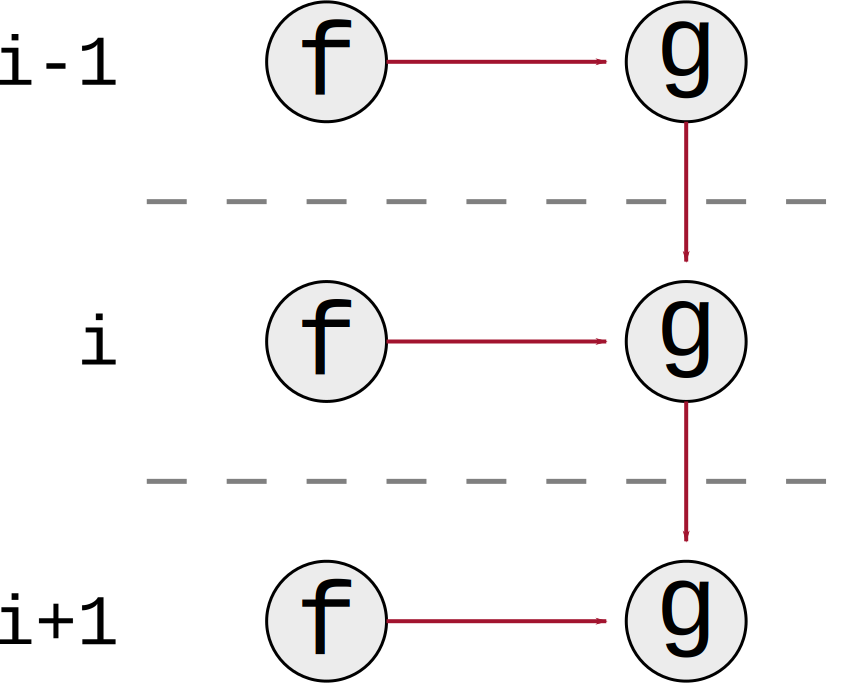
\includegraphics[width=0.7\textwidth]{figures/example_dag}
    \caption{\label{fig:dag-example}DAG corresponding to the
      sequential code presented in Figure~\ref{fig:stf-example}}
  \end{minipage}
  %% \caption{\label{fig:seq-example} Simple example of a sequential code
  %%   on the left with the corresponding DAG represented on the right.}
\end{figure}

As an example, we consider the sequential code in
Figure~\ref{fig:seq-example} for which the corresponding DAG is
represented in Figure~\ref{fig:dag-example}. Based on a STF model, the
parallel version of this code is illustrated in
Figure~\ref{fig:stf-example}. In the sequential code, the two
functions \textit{f} and \textit{g} manipulate arrays \textit{x} and
\textit{y}. The STF code is obtain by submitting the tasks that
consists of a kernels funtion (\textit{f} or \textit{g} in this
example) together with a data which is associated with a data access
which can possibly be \textit{R} when the data is read, \textit{W}
when the data is modified and \textit{RW} when the data is read and
modified.

As we have seen with this simple example is that the STF model is
extremely easy to exploit and this characteristic is certainly one of
the main reason for its extreme popularity in the HPC community. This
model, however, has several drawbacks that may affect the performance
and scalability of parallel codes relying on it. First the task are
issued and submitted to the runtime system sequentially. In the case
where, for a given DAG, the task granularity is small compared to the
time needed for building and submitting a task, the parallel execution
might be constraint by the time spent in the submission loop that is
setting up the DAG. To avoid this issue, it might be interesting to
consider a \textit{recursive} model where tasks might be used to
submit other tasks enabling the distribution of the cost for building
the DAG between the resources instead of doing it in a single
submission loop. This might be implemented for example with
\textit{callback} functions that are executed upon task completion and
can be use for the submission of tasks depending on the task that just
finished its execution. Another issue arising with the STF model comes
from the fact that the whole DAG is unrolled during the parallel
execution and every tasks in the DAG is stored in order to track task
dependencies. In the case where the DAG is extremely large, handling
and storing the DAG might represent an important overhead in terms of
computational cost and memory storage. Regarding this issue, even if
the recursive model allows to mitigate the problem, it my be necessary
to consider a radically different model such a the Parametrized Task
Graph (PTG) model which is introduced in~\cite{c.l:95}. In this model,
task dependencies are explicitly encoded according to the data-flow of
each task and as a results the whole DAG can be expressed in a compact
format. 

%% In the present paper we mainly focus on the 

\section{Runtime systems}\label{sec:runtime}
\setcounter{equation}{0}
\setcounter{table}{0}
\setcounter{figure}{0}

The popularity of task-based algorithms push the OpenMP standard to
introduce the \textit{task} construct in the version 3.0 its API. Then
motivated by the popularity of the STF model, the OpenMP board decided
to include the \textit{depend} construct in the version 4.0 allowing
users to express dependencies between tasks in a way complying with
the STF model. In this work we propose an OpenMP implementation of our
Cholesky solver and show advantages of using this standard in terms of
performance, scalability and productivity. However because many
features are still unavailable in the standard we also developed
another version based on the StarPU runtime system. Both
implementations of our solver rely on a STF model, but the
StarPU-based implementation might benefit from a wider range of
feature available with StarPU. For example, although we focus on
shared-memory architectures in this work, the StarPU version might be
extended into a distributed-memory version whereas OpenMP doesn't
provide any possibility to run on distributed memory architectures.

In order to introduce the features provided by StarPU API and the
features provided by this runtime system, we show in
Figure~\ref{fig:seq-starpu-example} an example of a StarPU-based
implementation for the simple example presented in
Figure~\ref{fig:seq-example}. The task submission is done through the
\texttt{starpu\_task\_insert} function that tasks in input a
\textit{codelet} and a set of \textit{handles}. A codelet correspond
to the description of a task and include a list of computational
resources where the task can be executed as well as the corresponding
computational kernels. In our example the codelet \texttt{g\_cl}
describe a task that can be executed on a CPU and a CUDA device
(\texttt{STARPU\_CPU | STARPU\_CUDA}) respectively with the kernels
\texttt{g\_cpu\_func} and \texttt{g\_cuda\_func}. The data handles
represents a piece of data that is accessed in the task and can be
read (\texttt{STARPU\_R}), written (\texttt{STARPU\_W}) or read and
written (\texttt{STARPU\_RW}). In order to be accessed, a data handle
must be \textit{registered} to the runtime system by providing
information such as a pointer on the data, its size and type. These
information allows StarPU to automatically perform the data transfer
between the memory nodes during the execution. For example, when a
data needs to be accessed on a GPU device, the runtime system
automatically transfer it to the device memory node. As a results
StarPU is capable of ensuring the data consistency multiple
nodes. When all the tasks have been submitted to the runtime system,
we wait for their completion by calling the routine
\texttt{starpu\_task\_wait\_for\_all}.

\begin{figure}[!h]
  \lstset{language=C, procnamekeys={},escapechar=>}
  \centering \lstinputlisting{listings/stf-starpu-example.c}
  \caption{\label{fig:stf-starpu-example}Simple example of a parallel version
    of the sequential code in Figure~\ref{fig:seq-example} using a STF
    model with \starpu.}
\end{figure}

\section{Parallelisation of a task-based Cholesky factorization using a STF programming model}
\label{sec:experiments}



\begin{figure}[!h]
  \centering \lstinputlisting{listings/spllt_facto_stf.f90}
\caption{\label{fig:activation-pseudocode-1d}Pseudo-code for the
  sparse Cholesky factorization using a STF model.}
\end{figure}

\section{Experimental results}\label{sec:experiments}

\begin{table}[htbp]
    \begin{center}
      \begin{tabular}{l|rr|rr|rr}
  \hline
  Matrix                          & \multicolumn{4}{c}{spLLT}        & \multicolumn{2}{c}{MA87}                                         \\
  \hline
                                  & \multicolumn{2}{c}{OpenMP (gnu)} & \multicolumn{2}{c}{StarPU} & \multicolumn{2}{c}{MA87}            \\ 
  \cline{2-7}
                                  & nb                               & facto (s)                  & nb   & facto (s) & nb  & facto (s)  \\
  \hline
  Schmid/thermal2                 & 512                              & 1.801                      & 1024 & 2.123     & 256 & \bf 0.376  \\
  Rothberg/gearbox                & 256                              & \bf 0.220                  & 384  & 0.318     & 256 & 0.252      \\
  DNVS/m\_t1                      & 256                              & 0.205                      & 384  & 0.262     & 256 & \bf 0.194  \\
  Boeing/pwtk                     & 384                              & 0.241                      & 512  & 0.382     & 256 & \bf 0.235  \\
  Chen/pkustk13                   & 256                              & 0.222                      & 256  & 0.311     & 256 & \bf 0.220  \\
  GHS\_psdef/crankseg\_1          & 256                              & 0.254                      & 256  & 0.272     & 256 & \bf 0.242  \\
  Rothberg/cfd2                   & 256                              & 0.269                      & 384  & 0.350     & 256 & \bf 0.260  \\
  DNVS/thread                     & 256                              & \bf 0.203                  & 384  & 0.240     & 256 & 0.213      \\
  DNVS/shipsec8                   & 256                              & \bf 0.245                  & 384  & 0.330     & 256 & 0.250      \\
  DNVS/shipsec1                   & 256                              & \bf 0.247                  & 384  & 0.363     & 256 & 0.259      \\
  GHS\_psdef/crankseg\_2          & 256                              & 0.267                      & 384  & 0.310     & 256 & \bf 0.257  \\
  DNVS/fcondp2                    & 256                              & 0.334                      & 384  & 0.461     & 256 & \bf 0.271  \\
  Schenk\_AFE/af\_shell3          & 768                              & 0.546                      & 384  & 0.855     & 256 & \bf 0.424  \\
  DNVS/troll                      & 256                              & 0.433                      & 384  & 0.577     & 256 & \bf 0.377  \\
  AMD/G3\_circuit                 & 512                              & 2.631                      & 512  & 3.345     & 256 & \bf 0.586  \\
  GHS\_psdef/bmwcra\_1            & 256                              & 0.367                      & 384  & 0.408     & 256 & \bf 0.342  \\
  DNVS/halfb                      & 256                              & 0.437                      & 512  & 0.590     & 256 & \bf 0.372  \\
  Um/2cubes\_sphere               & 384                              & 0.476                      & 384  & 0.537     & 256 & \bf 0.323  \\
  GHS\_psdef/ldoor                & 384                              & 1.095                      & 768  & 1.618     & 256 & \bf 0.599  \\
  DNVS/ship\_003                  & 256                              & 0.405                      & 384  & 0.456     & 256 & \bf 0.364  \\
  DNVS/fullb                      & 384                              & 0.500                      & 512  & 0.603     & 256 & \bf 0.431  \\
  GHS\_psdef/inline\_1            & 384                              & 0.683                      & 512  & 0.927     & 256 & \bf 0.667  \\
  Chen/pkustk14                   & 384                              & 0.613                      & 384  & 0.635     & 256 & \bf 0.555  \\
  GHS\_psdef/apache2              & 512                              & 1.416                      & 512  & 1.848     & 256 & \bf 0.717  \\
  Koutsovasilis/F1                & 384                              & 0.812                      & 512  & 0.920     & 256 & \bf 0.786  \\
  Oberwolfach/boneS10             & 384                              & 1.186                      & 384  & 1.599     & 256 & \bf 1.111  \\
  ND/nd12k                        & 384                              & 1.478                      & 384  & \bf 1.405 & 384 & 1.498      \\
  JGD\_Trefethen/Trefethen\_20000 & 512                              & 3.692                      & 384  & \bf 2.406 & 512 & 3.829      \\
  ND/nd24k                        & 384                              & 5.379                      & 384  & \bf 5.076 & 384 & 5.498      \\
  Oberwolfach/bone010             & 384                              & 7.416                      & 768  & 7.392     & 384 & \bf 7.195  \\
  GHS\_psdef/audikw\_1            & 768                              & 10.650                     & 768  & 10.680    & 384 & \bf 10.642 \\
  \hline
\end{tabular}

    \end{center}
    \caption{Factorization times (second) obtained with MA87 and SpLLT
      (i.e. MA87\_starpu). The factorizations were run with the block
      sizes \texttt{nb=(256, 384, 512, 768, 1024)} on 28 cores and
      \texttt{nemin=32}. The lowest factorization times are
      represented in bold.}
\end{table}

\section{Concluding remarks}\label{sec:conclusions}
This report has described in detail the development of a new

 
\section*{Code Availability}
A development version of the Cholesky factorization software used in this 
paper may be checked out of
our source code repository using the following command:

\begin{verbatim}
   svn co -r612 http://ccpforge.cse.rl.ac.uk/svn/spral/branches/xxxxxxx
\end{verbatim}

This code has not yet been optimised and so is not yet
part of the HSL or SPRAL libraries that are we develop
and maintain at the Rutherford Appleton Laboratory (see
\url{http://www.hsl.rl.ac.uk/} and \url{http://www.numerical.rl.ac.uk/spral/}).

\clearpage
\bibliography{flipflapflopBib}

\appendix

\section{Test problems}\label{appendix}
\setcounter{equation}{0}
\setcounter{table}{0}
\setcounter{figure}{0}
\setcounter{table}{0}
\renewcommand{\thetable}{A.\arabic{table}}


In Table~\ref{Tbl:Problems} we list  our test problems along with 
their characteristics. The problems are from the 
University of Florida Sparse Matrix Collection  and are chosen 
to represent a wide range of sparsity structures.

\end{document}
